\subsection{Pesquisa de Campo}

A pesquisa foi realizada por meio de um questionário digital no Google Forms, divulgado em um grupo do Facebook relacionado à proteção animal. Na consulta realizada em outubro de 2026, o formulário reunia 48 respostas. O instrumento continha 52 questões, duas delas abertas e opcionais. Como algumas perguntas dependiam de respostas anteriores, o total válido variou: 25 respostas nas questões 10 a 12, 31 na questão 14, 31 na questão aberta 15 e 40 na questão aberta 51. Os gráficos reproduzidos neste capítulo e no Apêndice B são cópias das visualizações originais do Google Forms; o número válido de cada questão aparece no próprio gráfico.

A amostra foi não probabilística, por conveniência, formada por pessoas que decidiram responder ao formulário. Assim, os resultados descrevem somente o grupo consultado e não permitem generalização estatística. A concentração geográfica também deve ser considerada: 35 dos 48 participantes (72,9\%) residiam em Pelotas; quatro informaram Capão do Leão, três Rio Grande e dois cada Canguçu, Morro Redondo e Porto Alegre. Todos assinalaram ter 18 anos ou mais e concordaram em participar.

O perfil revela participação de pessoas com vínculos variados com a proteção animal. Quarenta e dois participantes (87,5\%) declararam ter animais de estimação; 35 (72,9\%) indicaram cães e 27 (56,3\%), gatos, sendo possível marcar mais de uma espécie. A Figura~\ref{fig:pesquisa_identificacao} apresenta as formas de identificação utilizadas nos animais dos participantes.

\begin{figure}[H]
\centering
\caption{Formas de identificação utilizadas nos animais dos participantes}
\label{fig:pesquisa_identificacao}
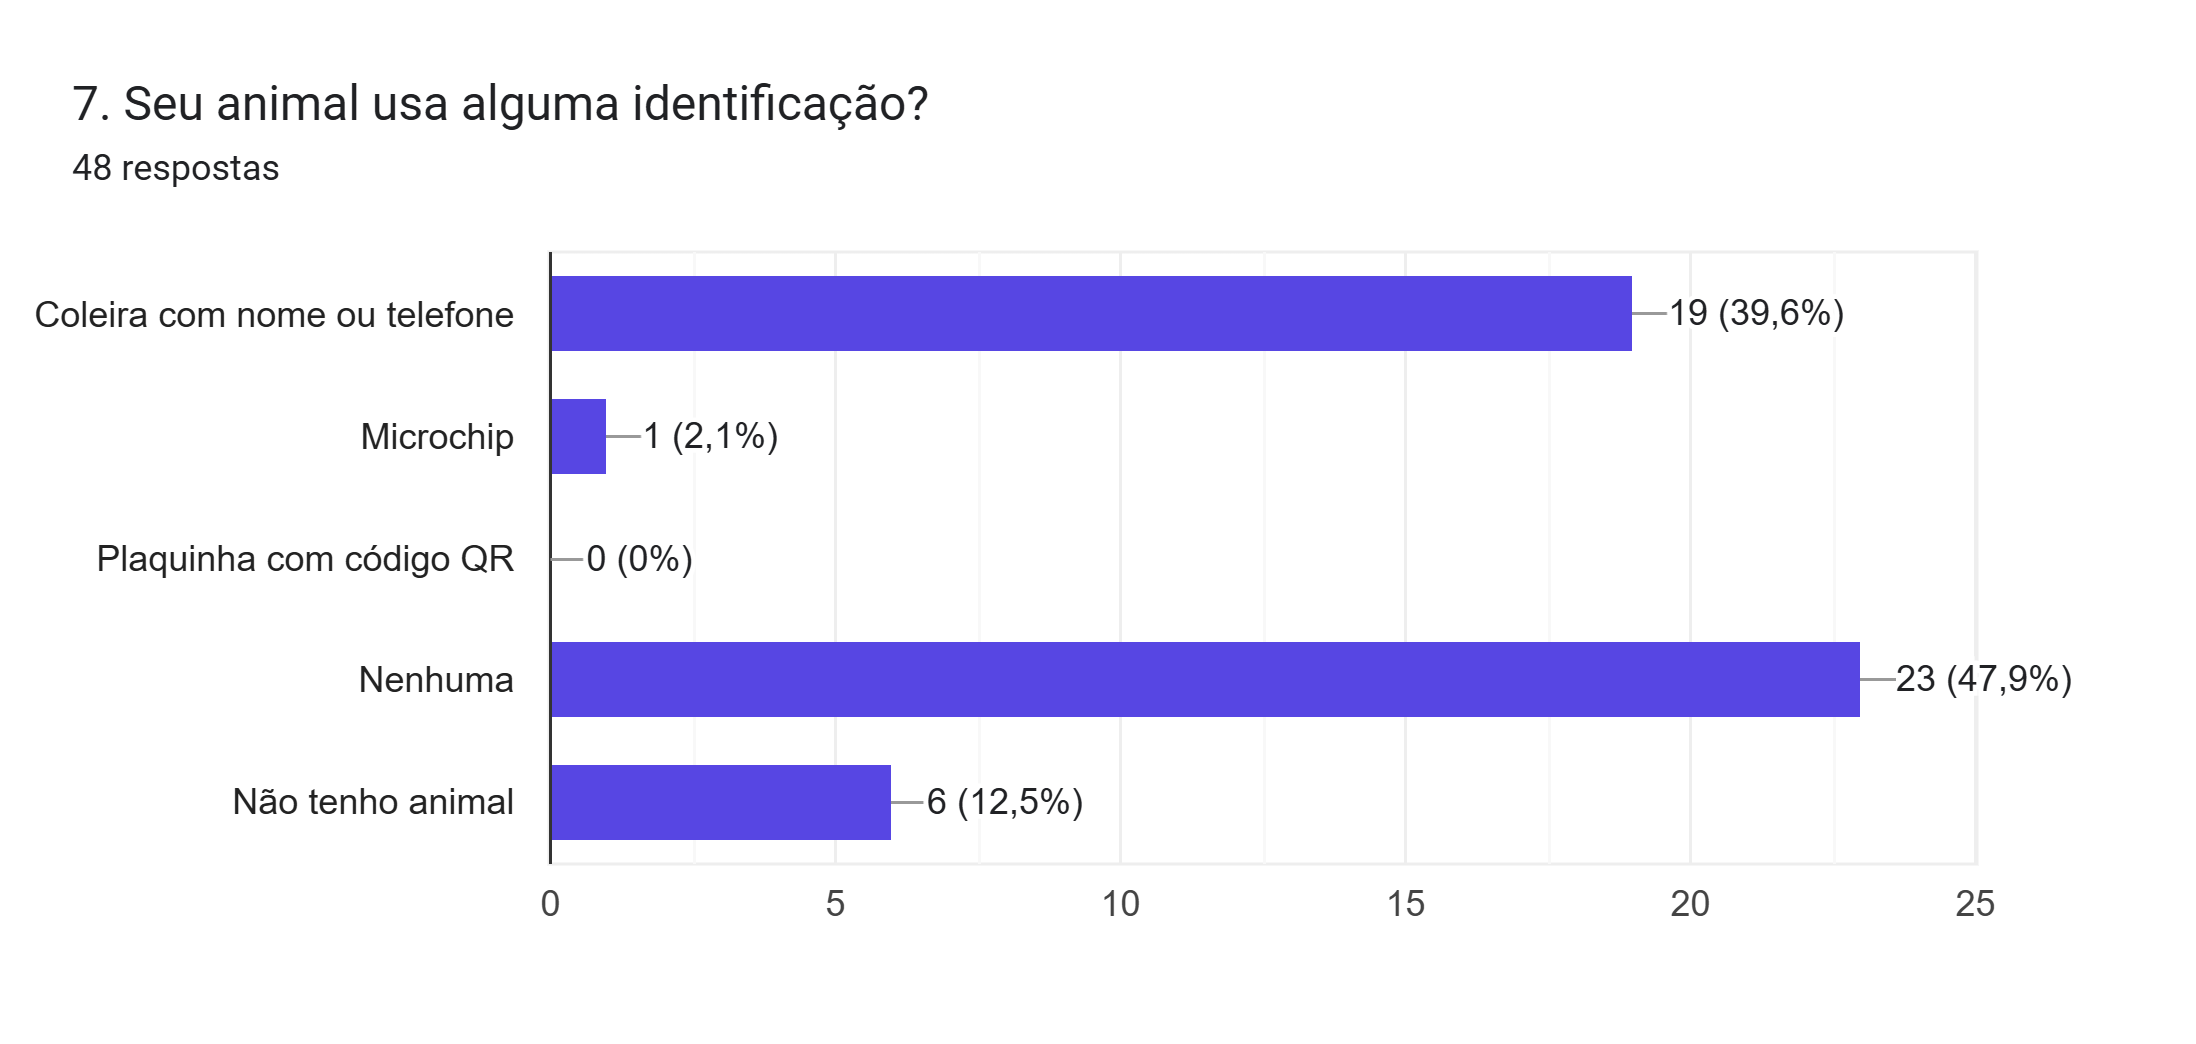
\includegraphics[width=\textwidth]{imagens/01_pesquisa/grafico_forms_q07.png}
\fonte{Google Forms (2026).}
\end{figure}

Na questão sobre identificação, 23 participantes (47,9\%) assinalaram não utilizar nenhuma das formas listadas, 19 (39,6\%) indicaram coleira com nome ou telefone e um (2,1\%) marcou microchip. As categorias não são mutuamente exclusivas.

A Figura~\ref{fig:pesquisa_animais_perdidos} apresenta as respostas sobre a experiência dos participantes com o desaparecimento de um animal próprio.

\begin{figure}[H]
\centering
\caption{Experiência dos participantes com o desaparecimento de um animal próprio}
\label{fig:pesquisa_animais_perdidos}
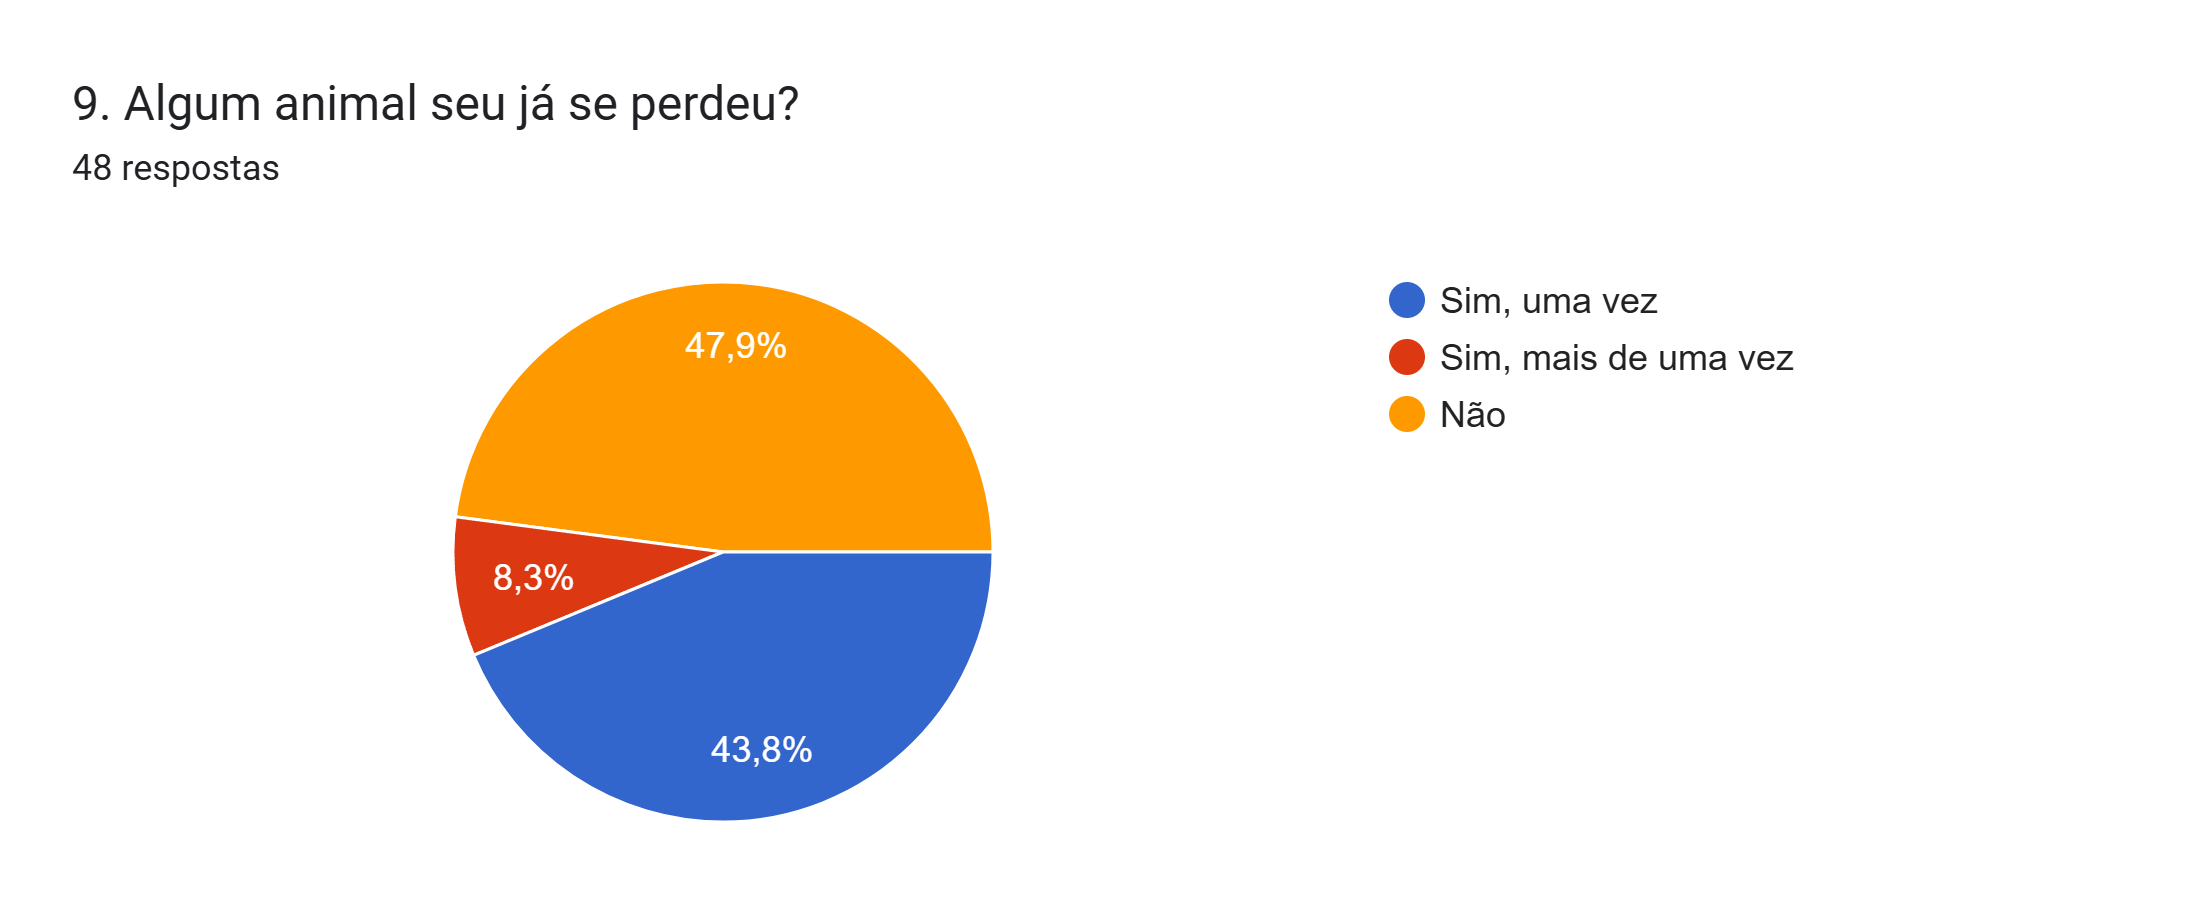
\includegraphics[width=\textwidth]{imagens/01_pesquisa/grafico_forms_q09.png}
\fonte{Google Forms (2026).}
\end{figure}

Vinte e cinco pessoas (52,1\%) relataram que um animal seu já havia se perdido uma ou mais vezes.

Entre esses participantes, a Figura~\ref{fig:pesquisa_tempo_reencontro} apresenta o tempo informado até o reencontro.

\begin{figure}[H]
\centering
\caption{Tempo até o reencontro do animal perdido}
\label{fig:pesquisa_tempo_reencontro}
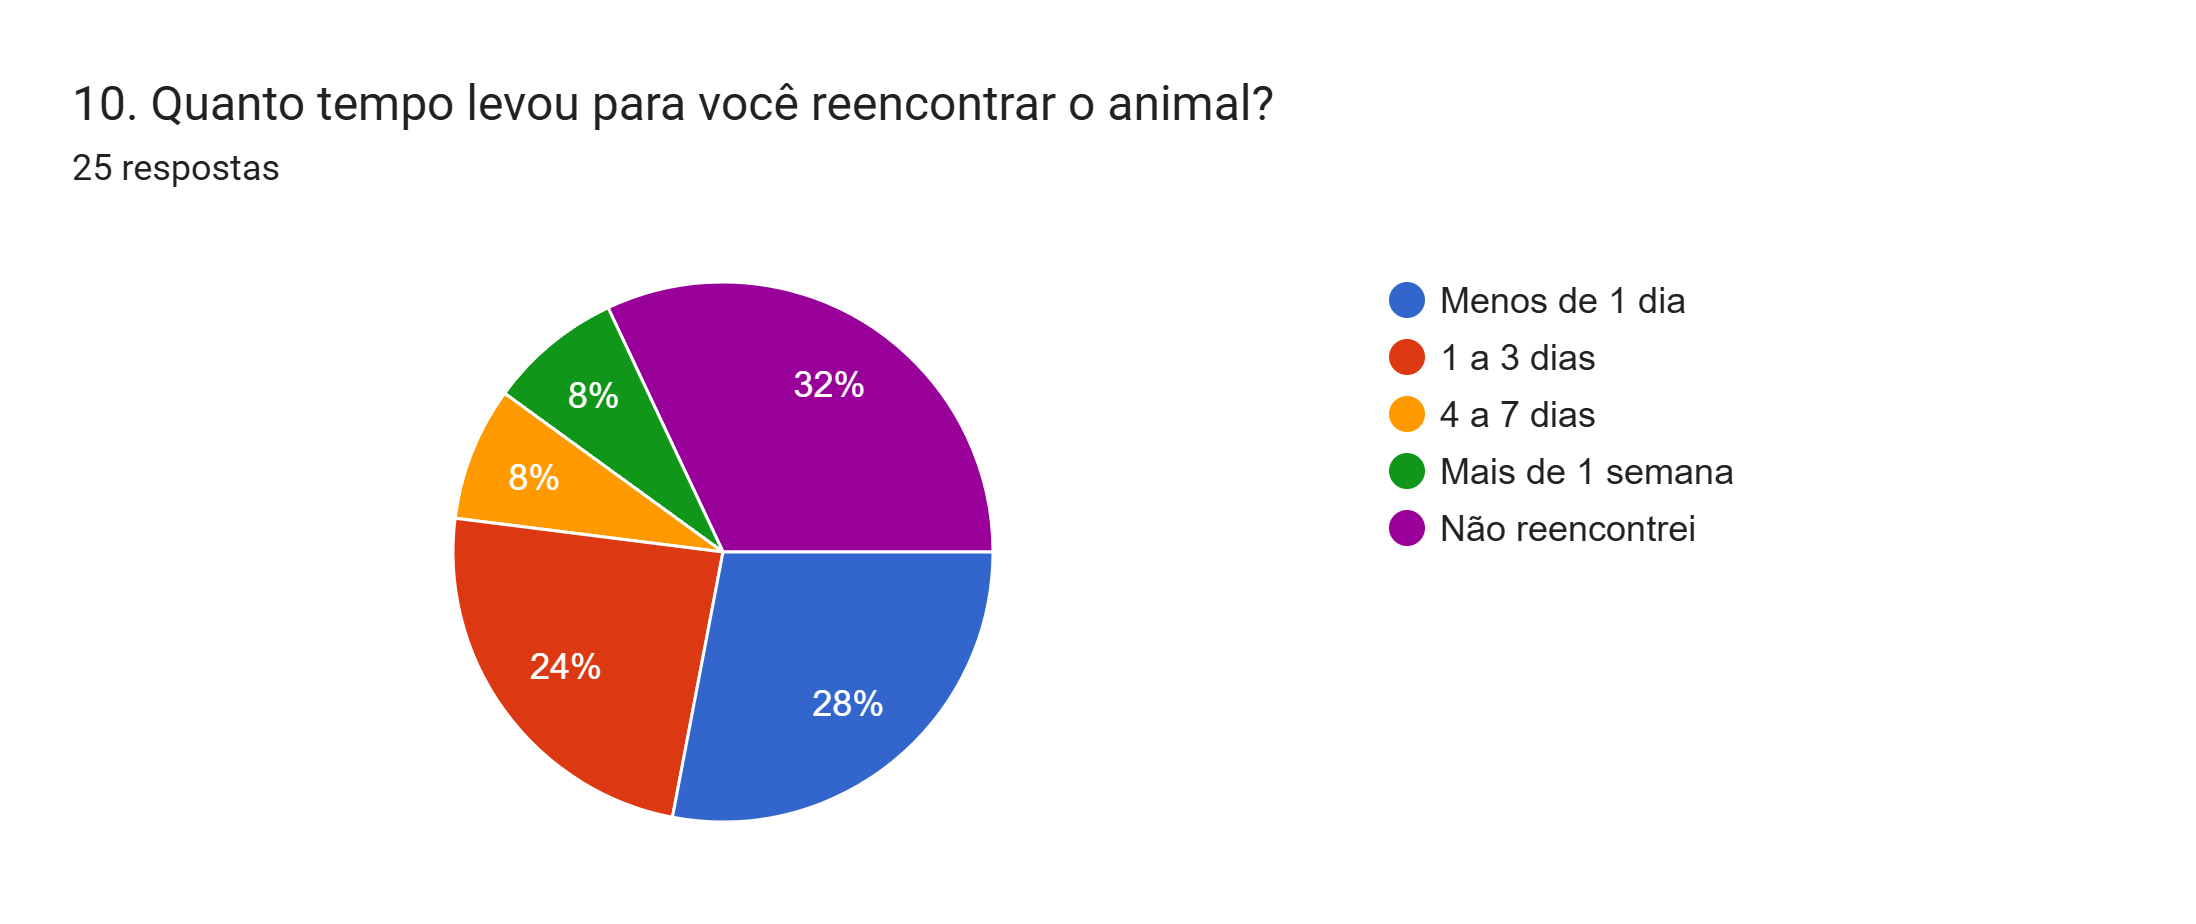
\includegraphics[width=\textwidth]{imagens/01_pesquisa/grafico_forms_q10.png}
\fonte{Google Forms (2026).}
\end{figure}

Sete participantes reencontraram o animal em menos de um dia, seis entre um e três dias, dois entre quatro e sete dias e dois depois de mais de uma semana; oito não o reencontraram.

A Figura~\ref{fig:pesquisa_meio_reencontro} mostra os meios indicados para reencontrar o animal, em uma questão respondida também por 25 participantes.

\begin{figure}[H]
\centering
\caption{Forma como o animal perdido foi reencontrado}
\label{fig:pesquisa_meio_reencontro}
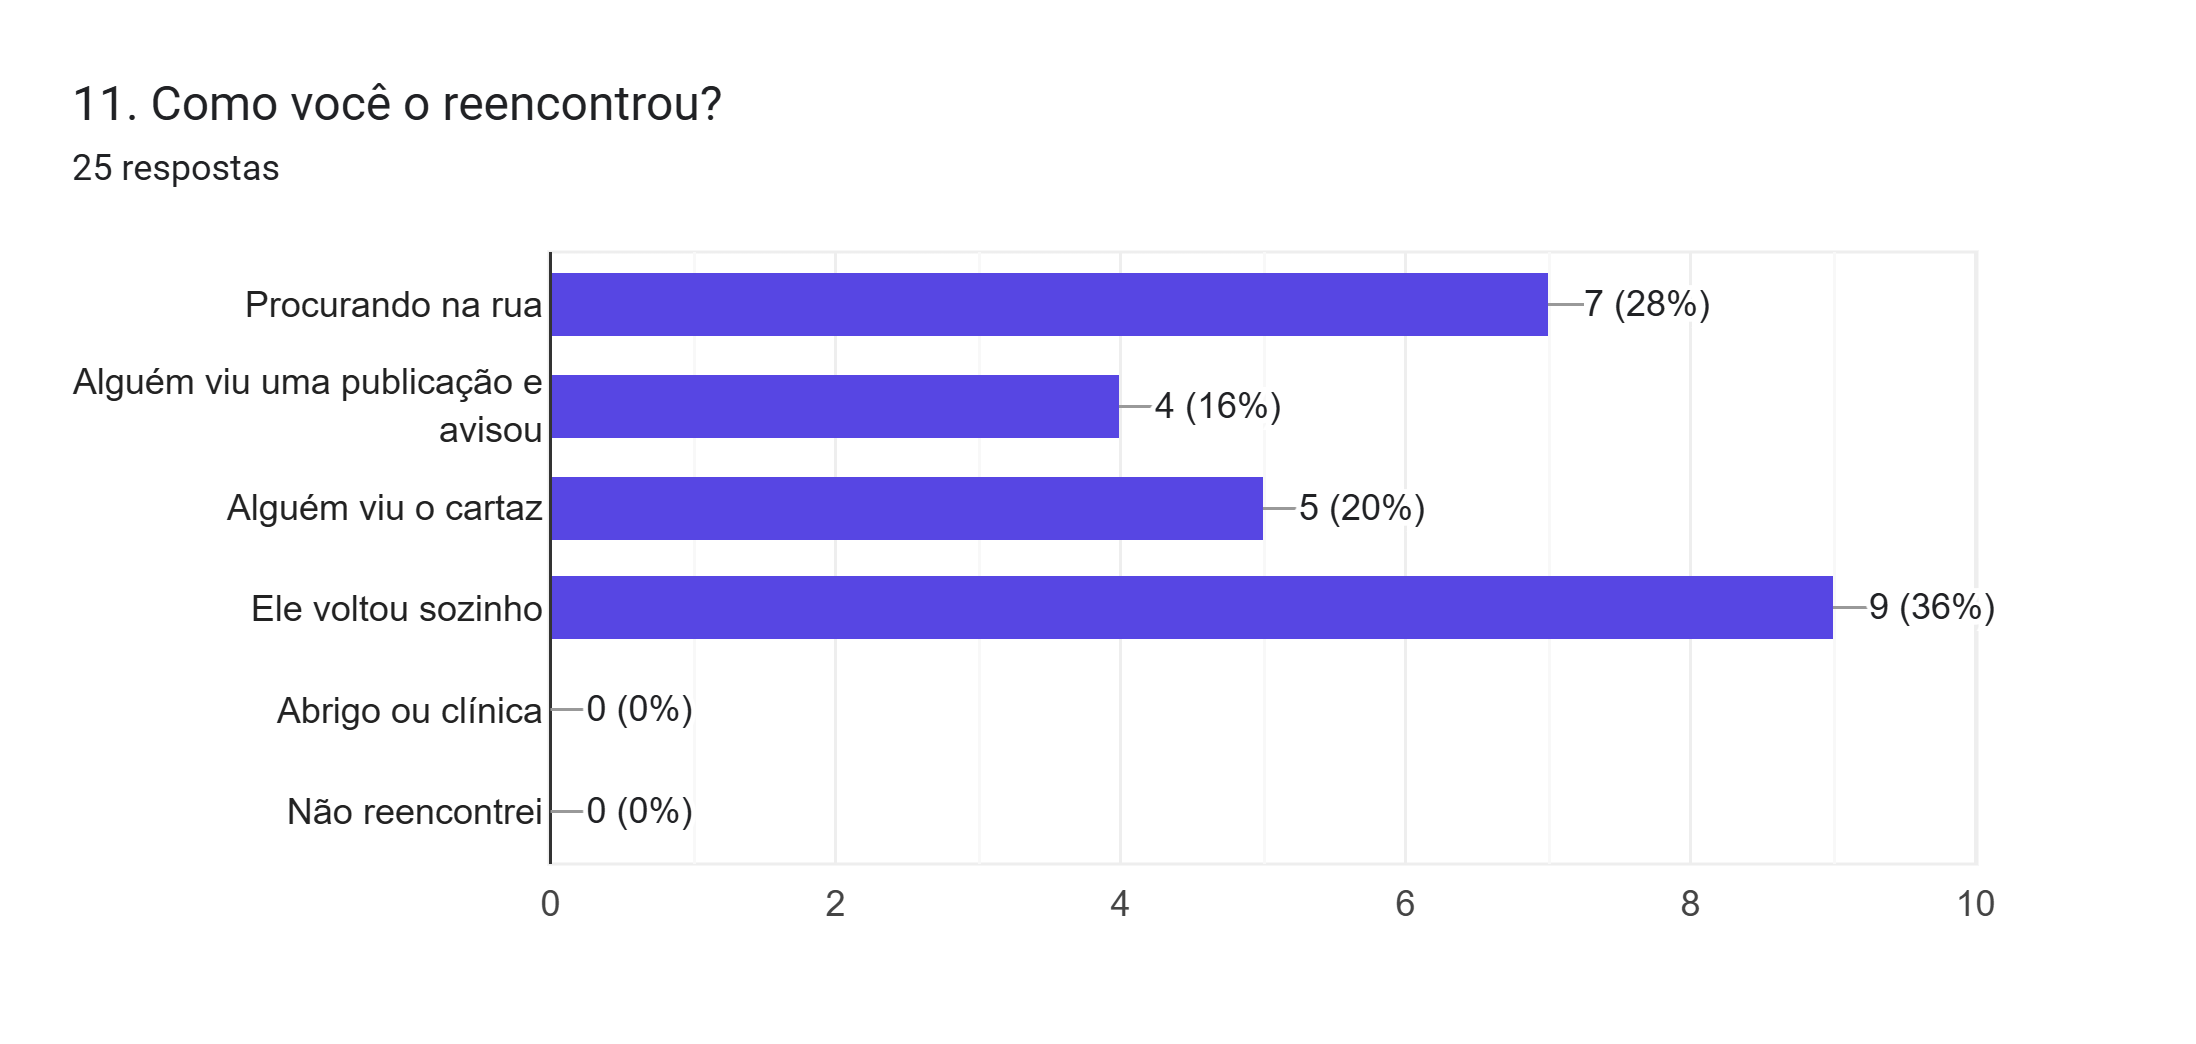
\includegraphics[width=\textwidth]{imagens/01_pesquisa/grafico_forms_q11.png}
\fonte{Google Forms (2026).}
\end{figure}

Nove participantes disseram que o animal voltou sozinho, sete que o encontraram procurando na rua, cinco que receberam aviso de alguém que viu o cartaz e quatro que foram avisadas por alguém que viu uma publicação. Nenhum marcou ``Não reencontrei'', embora oito tenham assinalado essa resposta na questão anterior. Como os dados agregados não permitem cruzar as respostas individuais, as distribuições são apresentadas separadamente, sem inferir como cada participante respondeu às duas questões.

As faixas etárias mais representadas foram de 25 a 34 anos (14 participantes; 29,2\%) e de 35 a 44 anos (12; 25\%); dez tinham de 45 a 59 anos (20,8\%), oito de 18 a 24 anos (16,7\%) e quatro 60 anos ou mais (8,3\%). Todos disseram usar o celular para redes sociais e mensagens ao menos uma vez por dia: 35 (72,9\%) várias vezes ao dia e 13 (27,1\%) uma vez ao dia. Os gráficos dessas questões de perfil estão no Apêndice B.

A Figura~\ref{fig:pesquisa_necessidades_iniciais} reúne as necessidades relatadas nas primeiras horas após o desaparecimento de um animal, na questão condicional respondida por 25 participantes.

\begin{figure}[H]
\centering
\caption{Necessidades relatadas nas primeiras horas após o desaparecimento de um animal}
\label{fig:pesquisa_necessidades_iniciais}
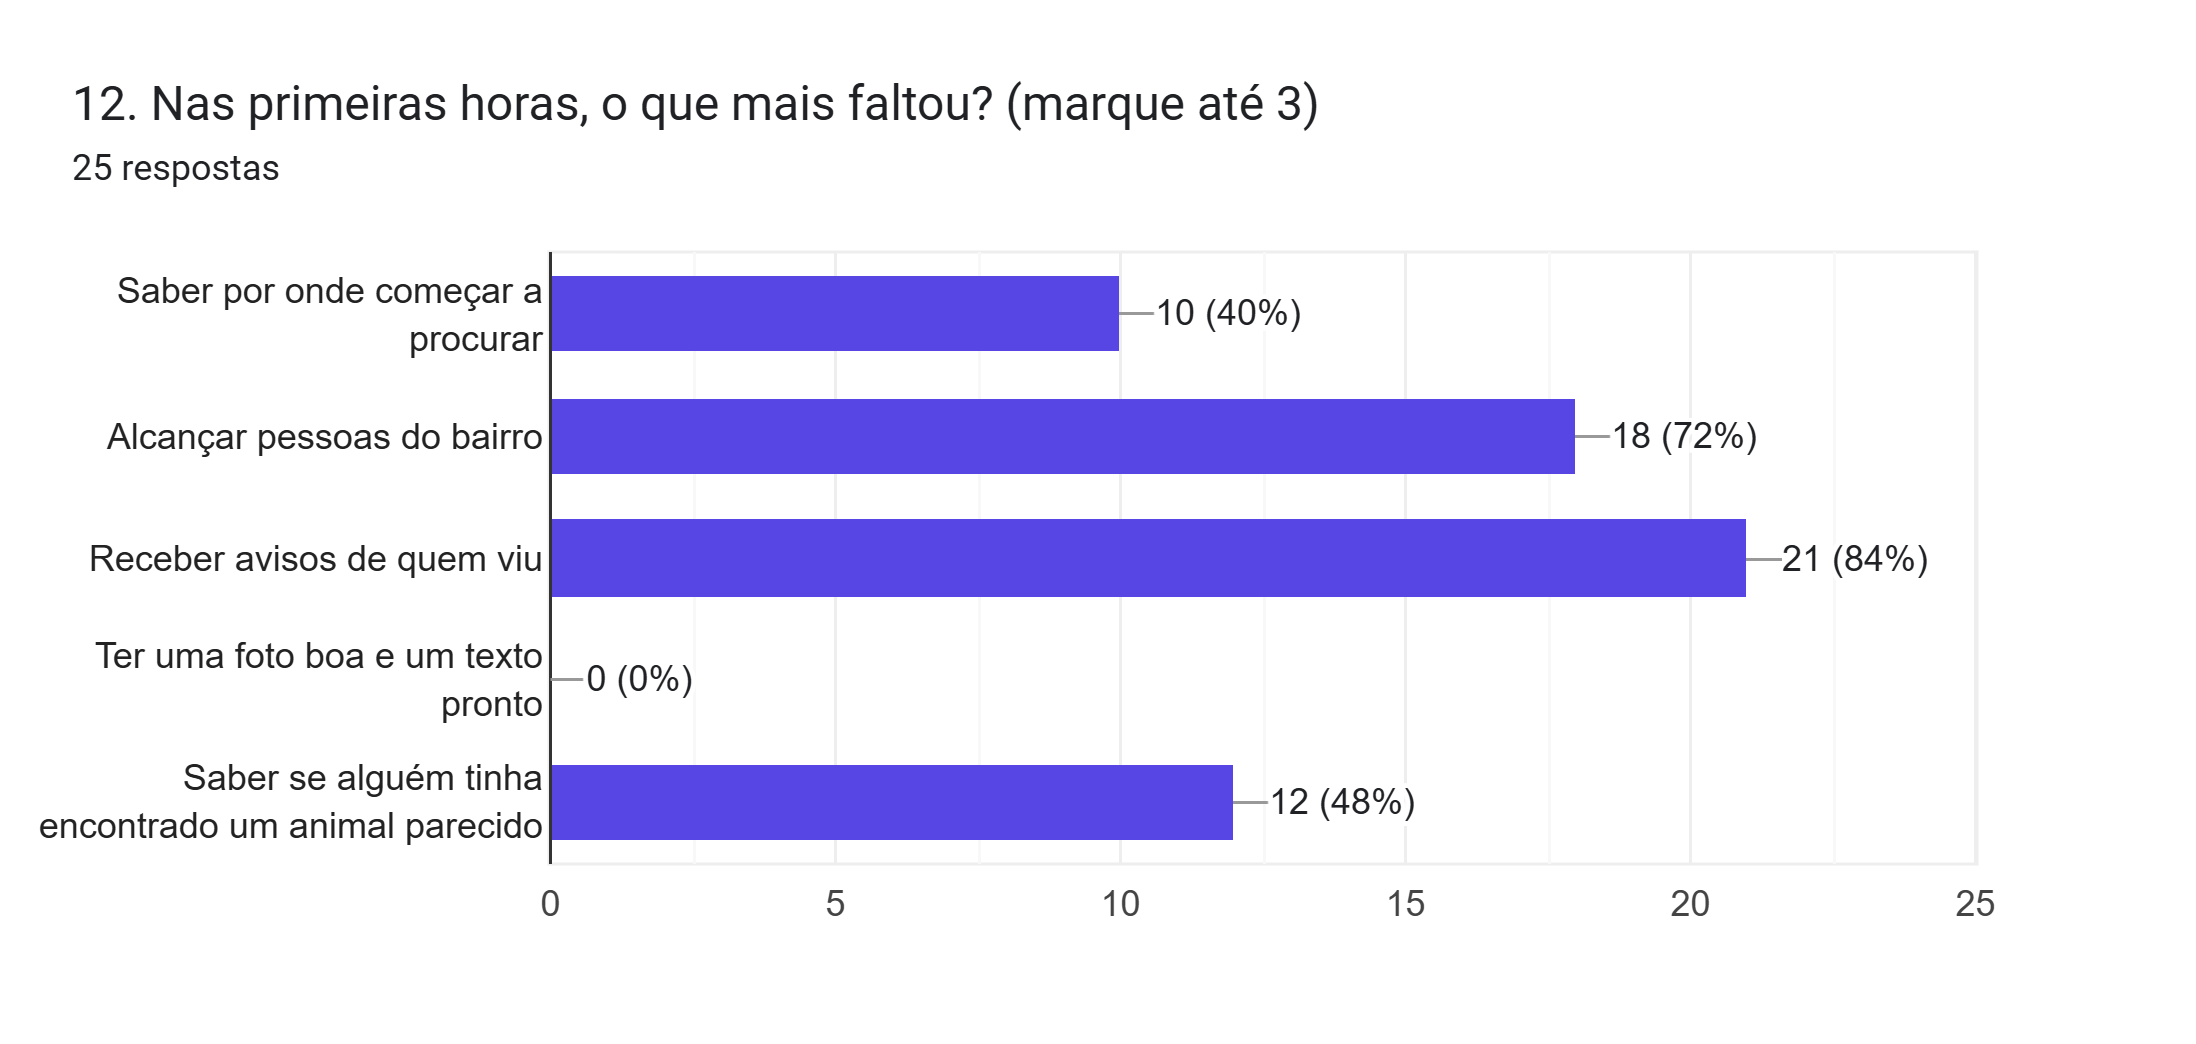
\includegraphics[width=\textwidth]{imagens/01_pesquisa/grafico_forms_q12.png}
\fonte{Google Forms (2026).}
\end{figure}

Vinte e um participantes (84\%) indicaram que faltou receber avisos de quem tivesse visto o animal; 18 (72\%) apontaram dificuldade para alcançar pessoas do bairro, dez (40\%) disseram não saber por onde começar e 12 (48\%) tiveram dificuldade para saber se alguém havia encontrado um animal parecido. Ninguém selecionou a necessidade de receber foto e texto prontos. A questão permitia até três seleções.

A Figura~\ref{fig:pesquisa_animais_encontrados} apresenta as respostas sobre a experiência de encontrar ou acolher animais.

\begin{figure}[H]
\centering
\caption{Experiência dos participantes ao encontrar ou acolher um animal}
\label{fig:pesquisa_animais_encontrados}
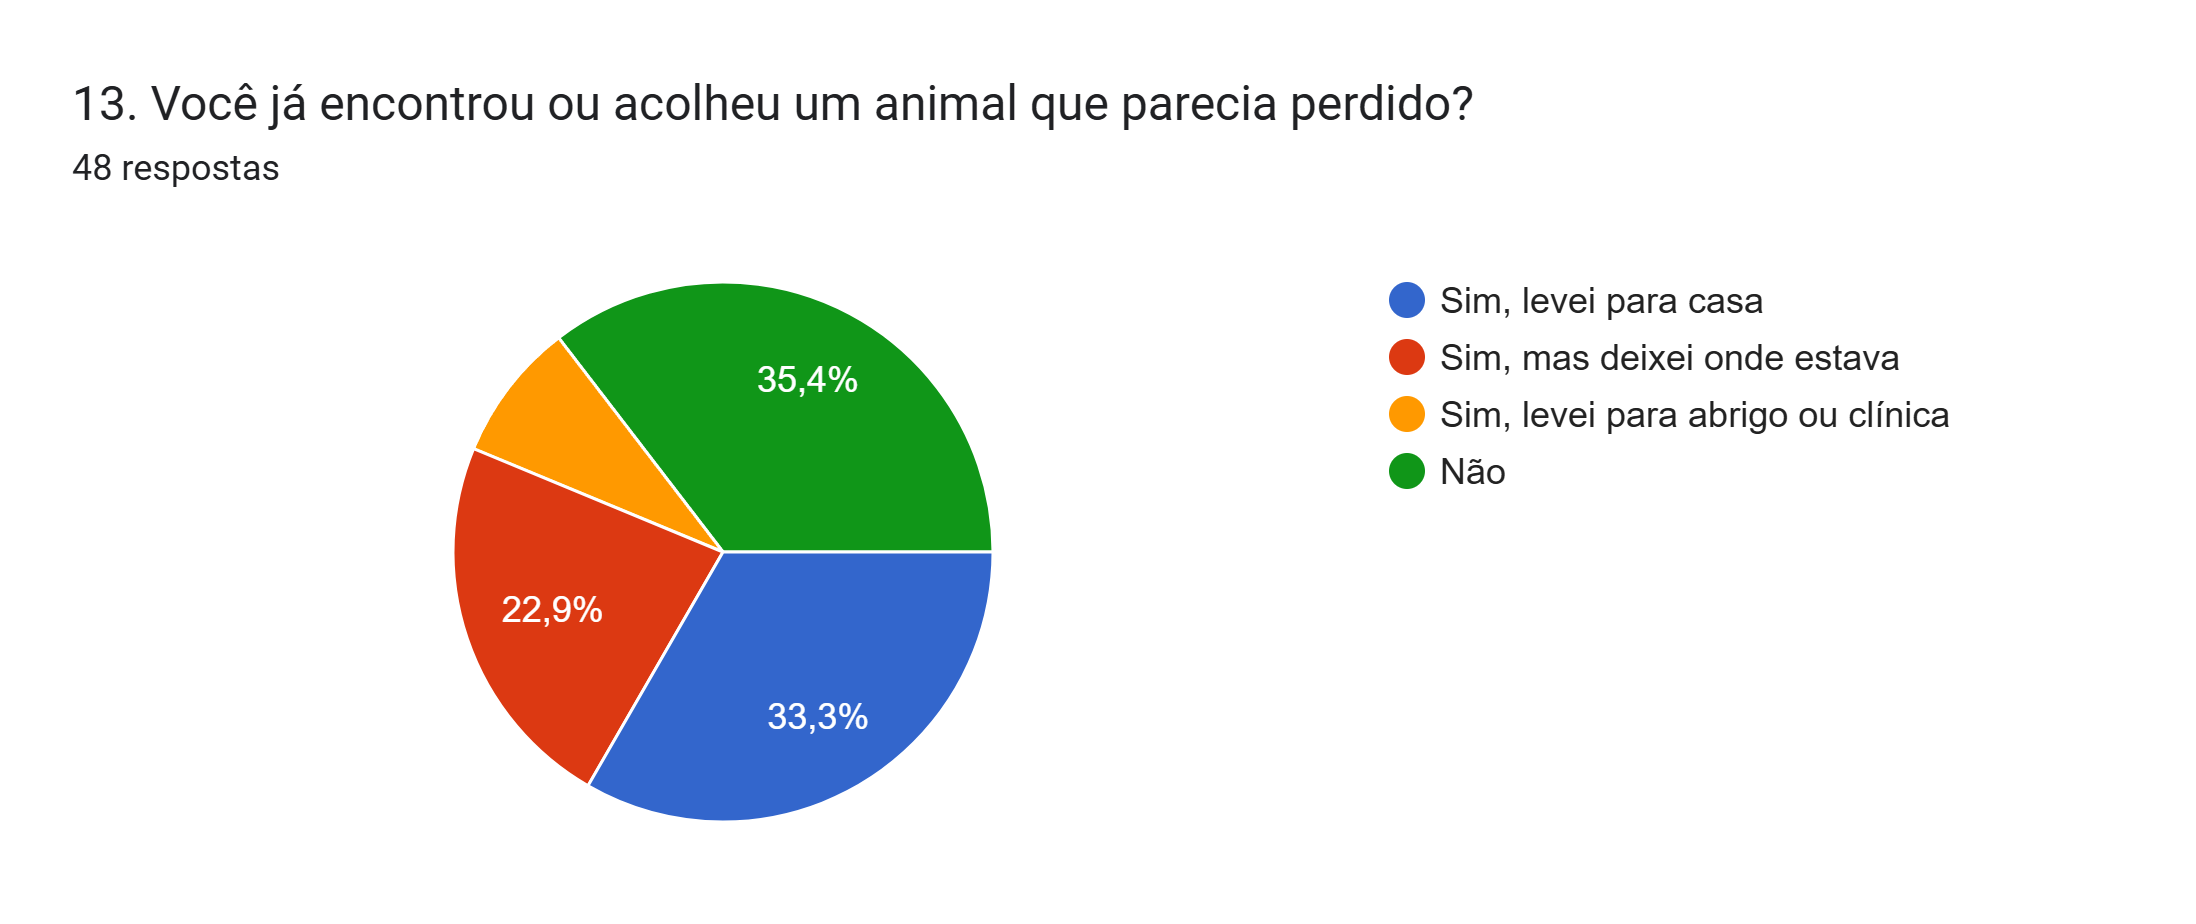
\includegraphics[width=\textwidth]{imagens/01_pesquisa/grafico_forms_q13.png}
\fonte{Google Forms (2026).}
\end{figure}

Trinta e um participantes (64,6\%) disseram já ter encontrado ou acolhido um animal: 16 o levaram para casa, 11 o deixaram onde estava e quatro o levaram a abrigo ou clínica.

A questão condicional seguinte, sobre como localizar o tutor, recebeu 31 respostas. Vinte participantes publicaram em rede social, 20 perguntaram aos vizinhos e 12 procuraram a leitura de microchip; 11 marcaram que não fizeram nada. Como eram permitidas múltiplas seleções, essas ações podem coexistir na mesma resposta.

A Figura~\ref{fig:pesquisa_canais_divulgacao} apresenta os canais que os participantes disseram utilizar para divulgar animais perdidos.

\begin{figure}[H]
\centering
\caption{Canais usados para divulgar animais perdidos}
\label{fig:pesquisa_canais_divulgacao}
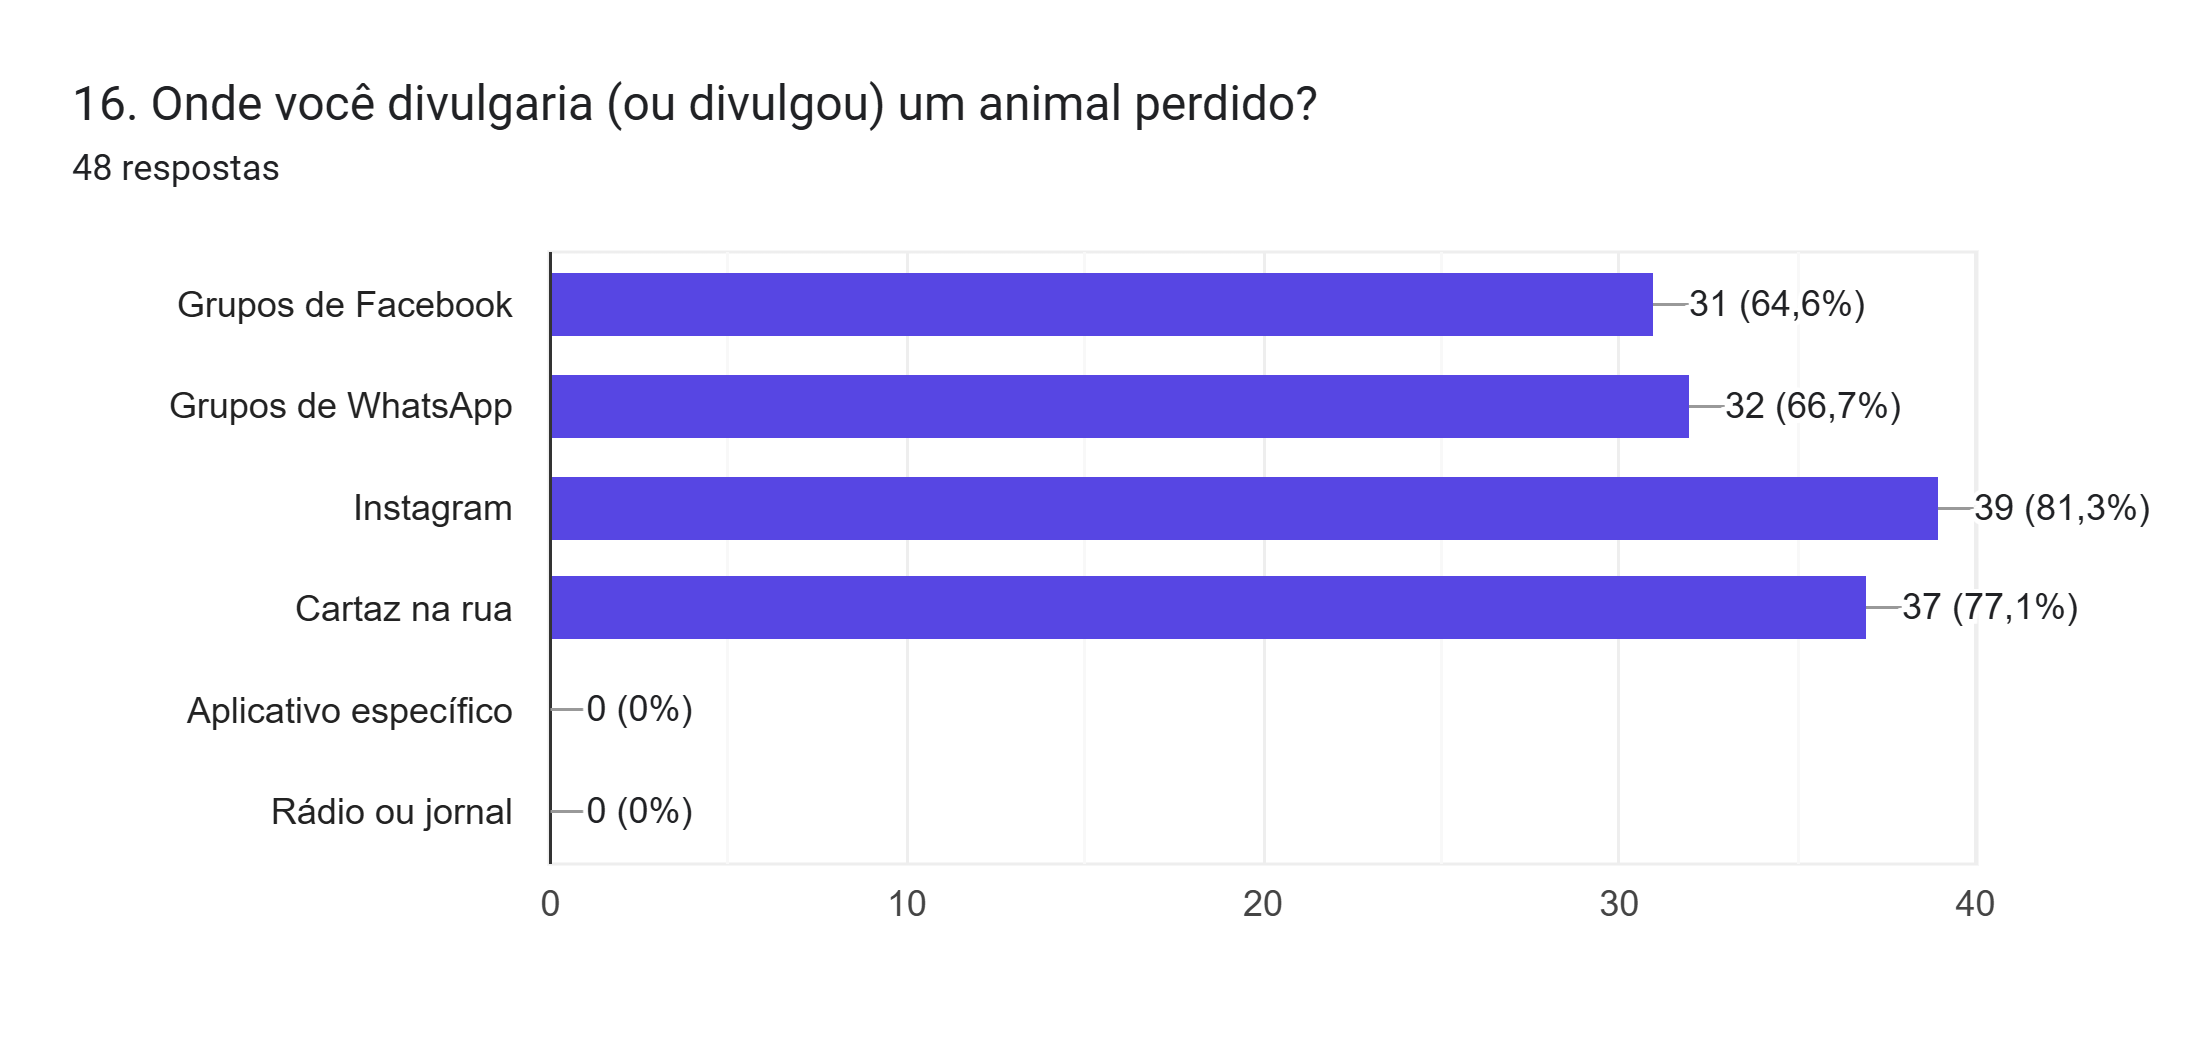
\includegraphics[width=\textwidth]{imagens/01_pesquisa/grafico_forms_q16.png}
\fonte{Google Forms (2026).}
\end{figure}

Instagram foi selecionado por 39 participantes (81,3\%), cartazes na rua por 37 (77,1\%), grupos de WhatsApp por 32 (66,7\%) e grupos de Facebook por 31 (64,6\%). A questão permitia mais de uma resposta.

A Figura~\ref{fig:pesquisa_dificuldades} apresenta as dificuldades percebidas nos canais de divulgação de animais perdidos.

\begin{figure}[H]
\centering
\caption{Dificuldades percebidas nos canais de divulgação de animais perdidos}
\label{fig:pesquisa_dificuldades}
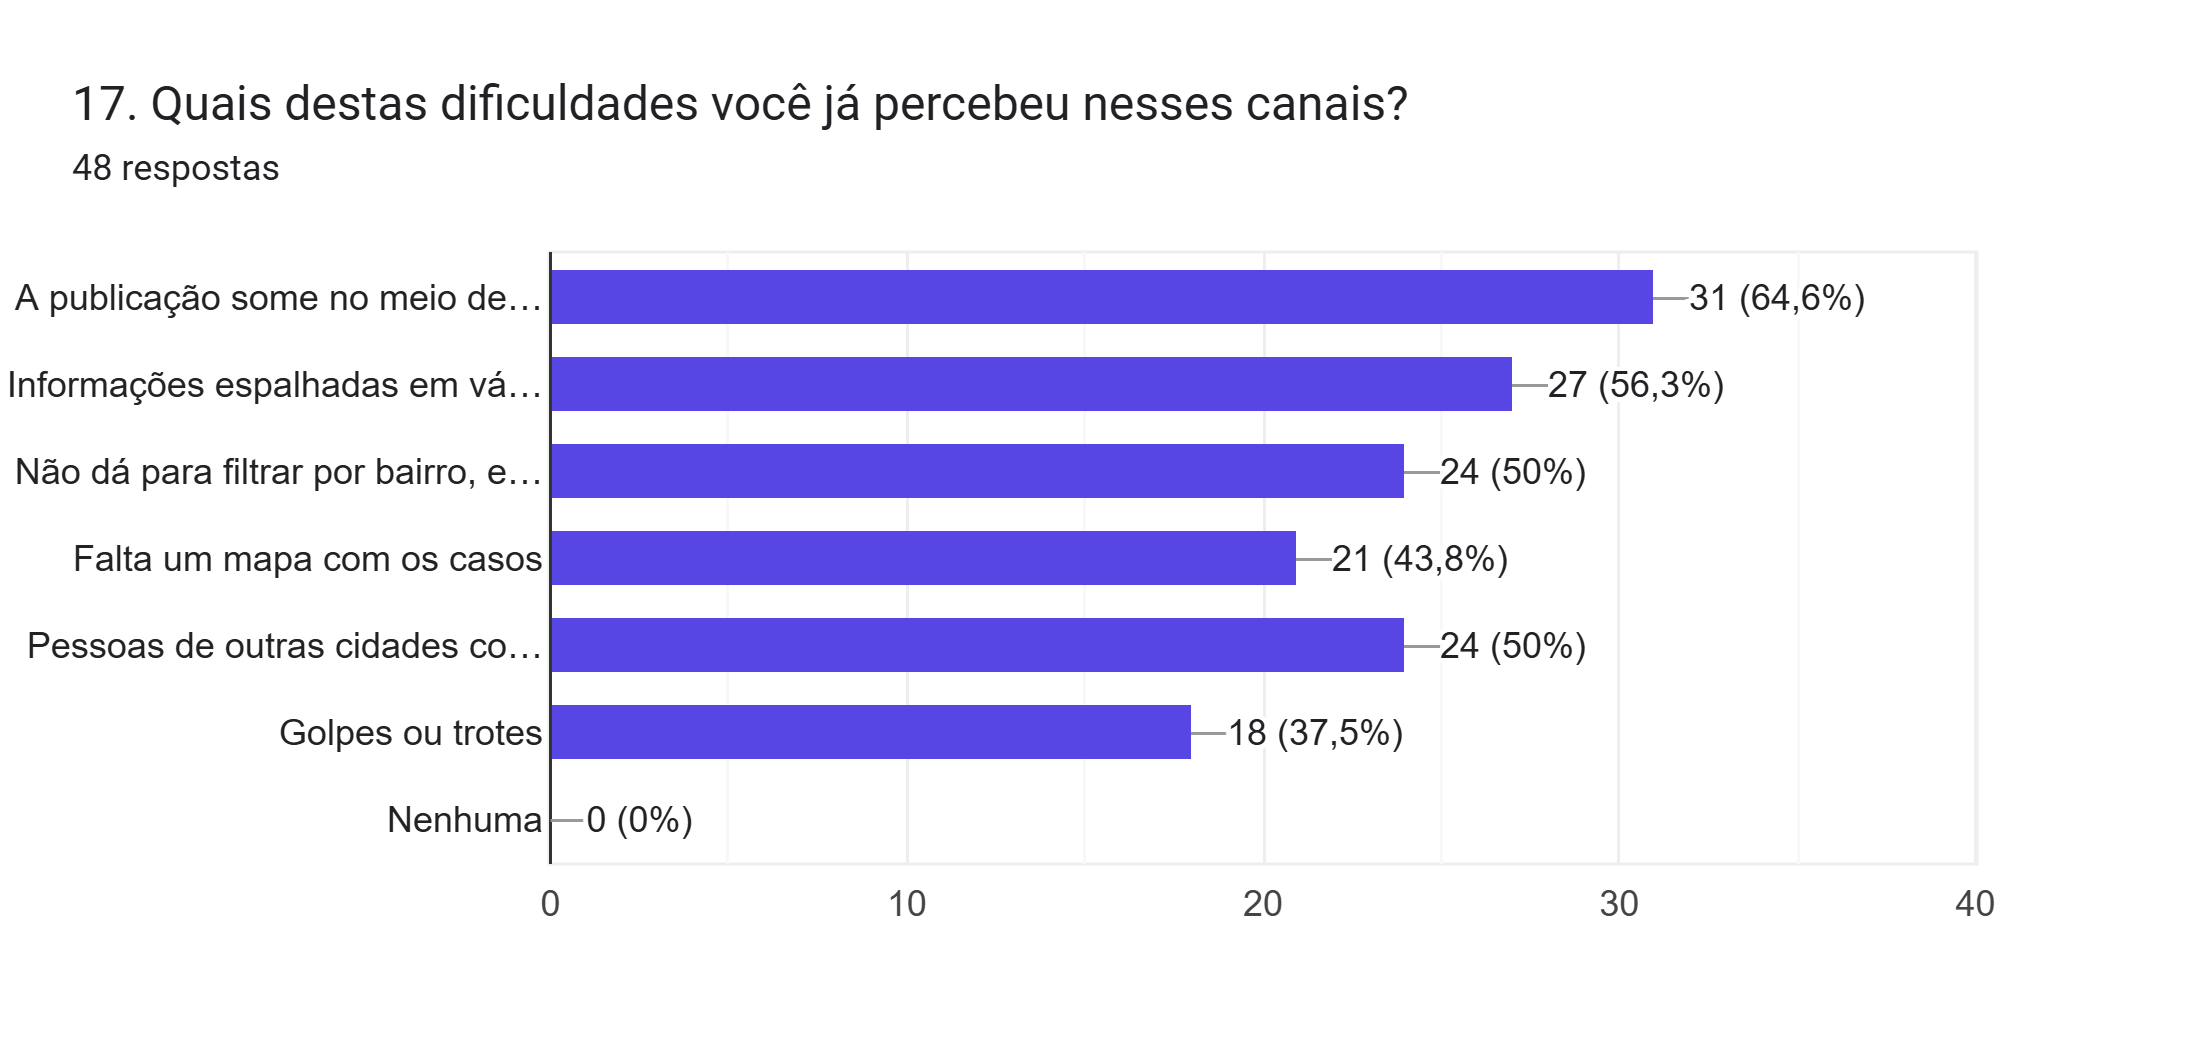
\includegraphics[width=\textwidth]{imagens/01_pesquisa/grafico_forms_q17_dificuldades.png}
\fonte{Google Forms (2026).}
\end{figure}

As dificuldades mais assinaladas foram as publicações desaparecerem entre outras (31; 64,6\%) e as informações ficarem espalhadas por vários grupos (27; 56,3\%). Também foram mencionados comentários de pessoas de outras cidades (24; 50\%), falta de filtros por bairro, espécie ou cor (24; 50\%), falta de mapa (21; 43,8\%) e golpes ou trotes (18; 37,5\%). A questão permitia múltiplas seleções; ninguém selecionou ``Nenhuma''.

A Figura~\ref{fig:pesquisa_utilidade_mapa} apresenta a avaliação dos participantes sobre a utilidade da visualização de animais em um mapa.

\begin{figure}[H]
\centering
\caption{Utilidade percebida da visualização de animais em mapa}
\label{fig:pesquisa_utilidade_mapa}
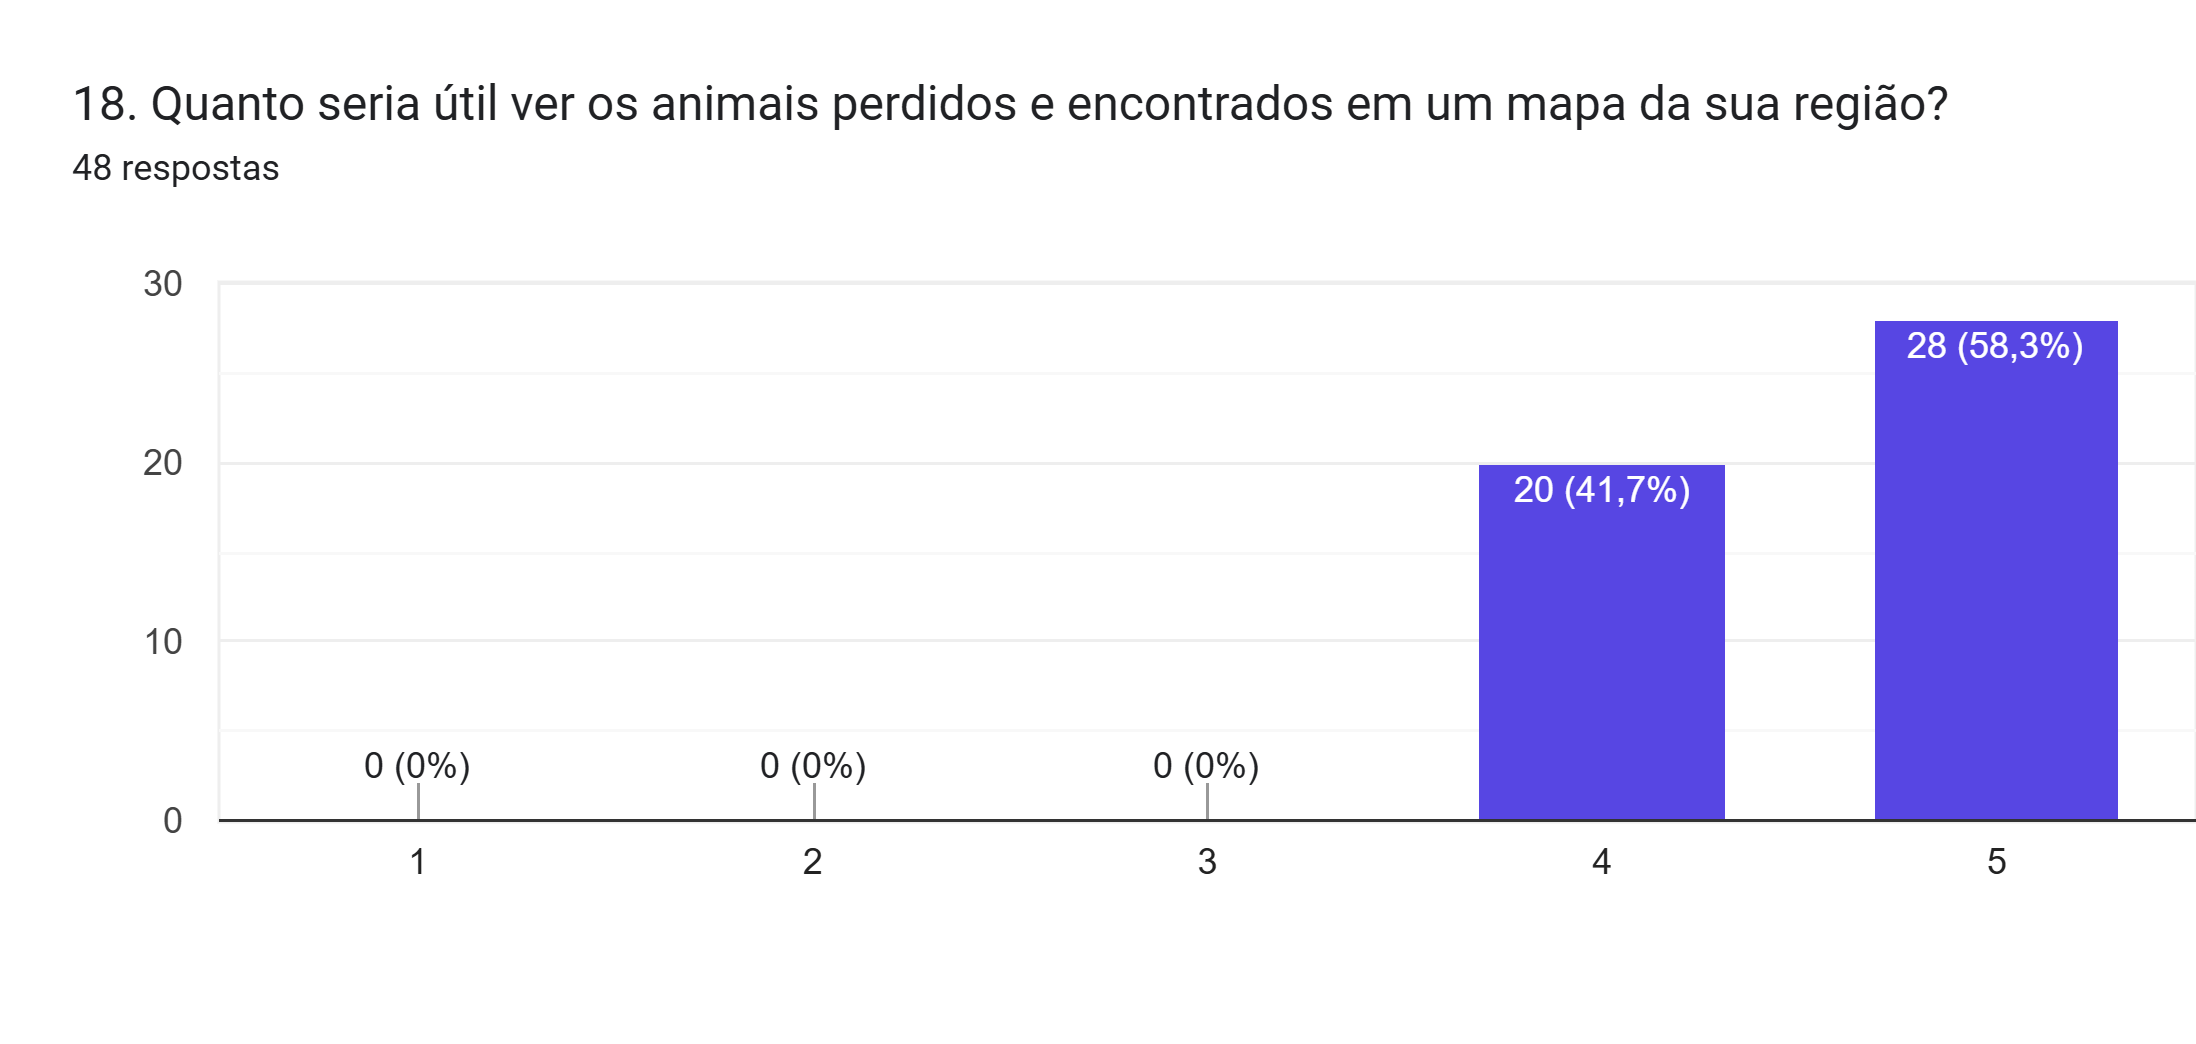
\includegraphics[width=\textwidth]{imagens/01_pesquisa/grafico_forms_q18_utilidade_mapa.png}
\fonte{Google Forms (2026).}
\end{figure}

A visualização em mapa foi avaliada com nota 4 por 20 participantes e nota 5 por 28; portanto, todos atribuíram uma das duas maiores notas. A mesma tendência apareceu na avaliação da priorização dos casos mais próximos: 21 deram nota 4 e 27, nota 5.

Para receber alertas de proximidade, 30 pessoas (62,5\%) preferiram o aplicativo e o WhatsApp, nove (18,8\%) somente o WhatsApp e nove (18,8\%) somente o aplicativo. Sobre a distância de busca no mapa, dez participantes escolheram 1 km, nove escolheram 3 km, 17 escolheram 5 km e 12 preferiram qualquer distância dentro da cidade. Espécie, cor, porte e bairro foram selecionados por todos como características de busca; raça por 27 (56,3\%), sexo e data do desaparecimento por 21 (43,8\%) cada. Ninguém selecionou idade. Essa questão permitia selecionar mais de uma característica.

As respostas também apontam limites práticos para a colaboração. Quarenta participantes (83,3\%) aceitariam gastar até três minutos para publicar um alerta; 32 (66,7\%) gastariam até um minuto para registrar um avistamento. Ao ver um animal parecido com um anúncio, 27 (56,3\%) avisariam o tutor pelo aplicativo com a localização, 12 (25\%) comentariam na publicação e nove (18,8\%) tirariam uma foto para enviar a alguém. Sobre a duração da utilidade de um avistamento, 18 participantes (37,5\%) escolheram ``Até 1 dia'', 12 (25\%) ``Mais de 2 dias'', 12 (25\%) ``Até 6 horas'' e seis (12,5\%) ``Até 2 dias''. A linha do tempo dos avistamentos recebeu notas 4 ou 5 de todos os participantes; a rota até o último local recebeu essas notas de 32 (66,7\%), enquanto 16 (33,3\%) atribuíram nota 3. A questão sobre deslocamento permitia múltiplas escolhas: deslocamento a pé foi marcado por 21 (43,8\%), carro ou moto por 20 (41,7\%), bicicleta por 16 (33,3\%) e ônibus por 16 (33,3\%).

Privacidade e confiança aparecem de forma recorrente nas respostas. A Figura~\ref{fig:pesquisa_privacidade_telefone} apresenta as notas atribuídas ao incômodo de deixar o telefone visível em uma publicação pública.

\begin{figure}[H]
\centering
\caption{Incômodo com a exposição pública do telefone pessoal}
\label{fig:pesquisa_privacidade_telefone}
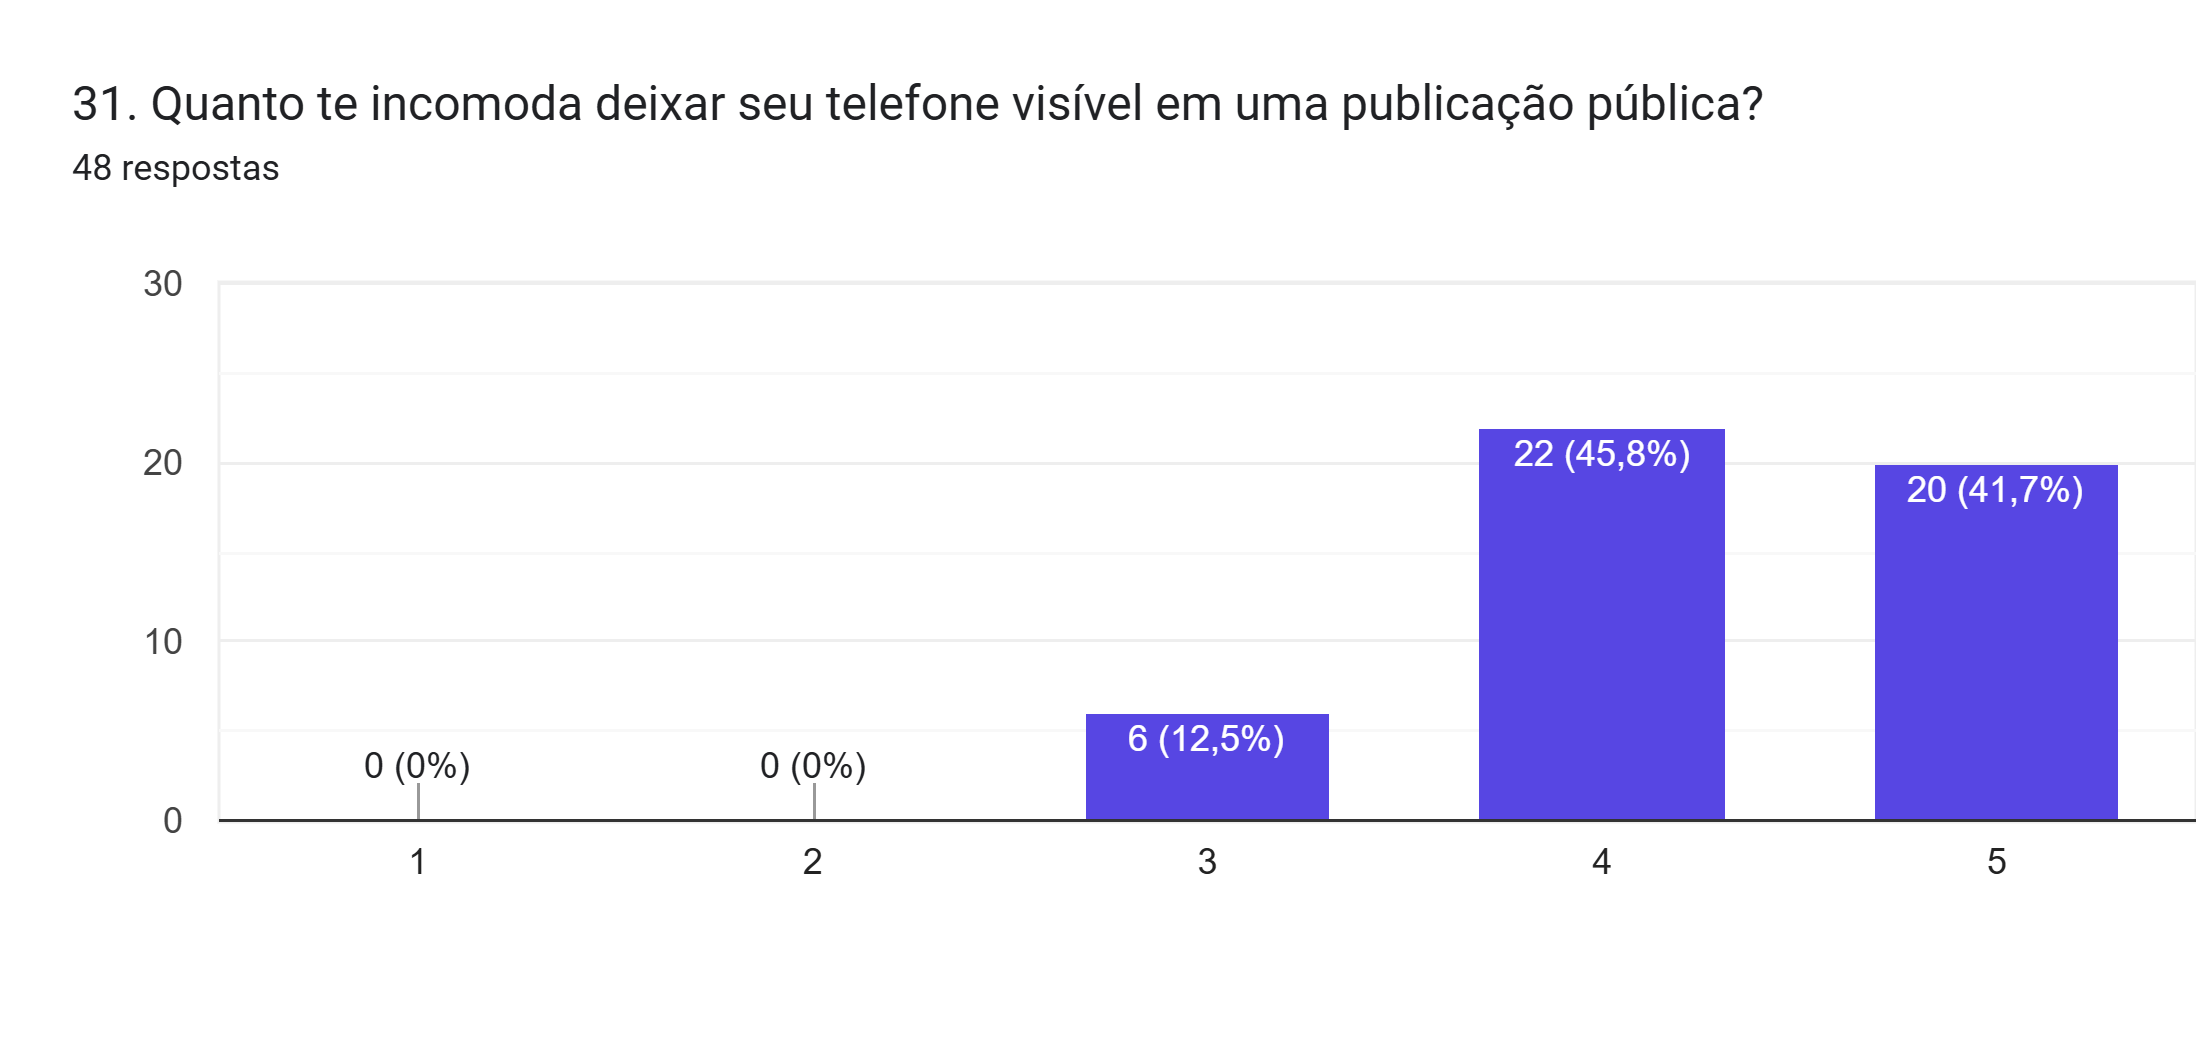
\includegraphics[width=\textwidth]{imagens/01_pesquisa/grafico_forms_q31_privacidade_telefone.png}
\fonte{Google Forms (2026).}
\end{figure}

Vinte e dois participantes atribuíram nota 4 e 20, nota 5 a esse incômodo. Sobre experiências anteriores de divulgação, 30 (62,5\%) relataram trotes, golpes ou contatos insistentes; 12 (25\%) nunca haviam divulgado e seis (12,5\%) não receberam esse tipo de contato. O canal de contato preferido foi o chat do aplicativo sem exposição do telefone (23; 47,9\%), seguido da indiferença entre os dois canais (14; 29,2\%) e do WhatsApp (11; 22,9\%). Em cartazes, 24 participantes (50\%) só divulgariam o WhatsApp se pudessem escolher em cada caso, cinco (10,4\%) o incluiriam sempre e 19 (39,6\%) prefeririam um código QR para o aplicativo.

A Figura~\ref{fig:pesquisa_privacidade_local} apresenta as preferências sobre a localização a exibir quando um animal encontrado está acolhido.

\begin{figure}[H]
\centering
\caption{Preferência de exposição do local onde um animal foi acolhido}
\label{fig:pesquisa_privacidade_local}
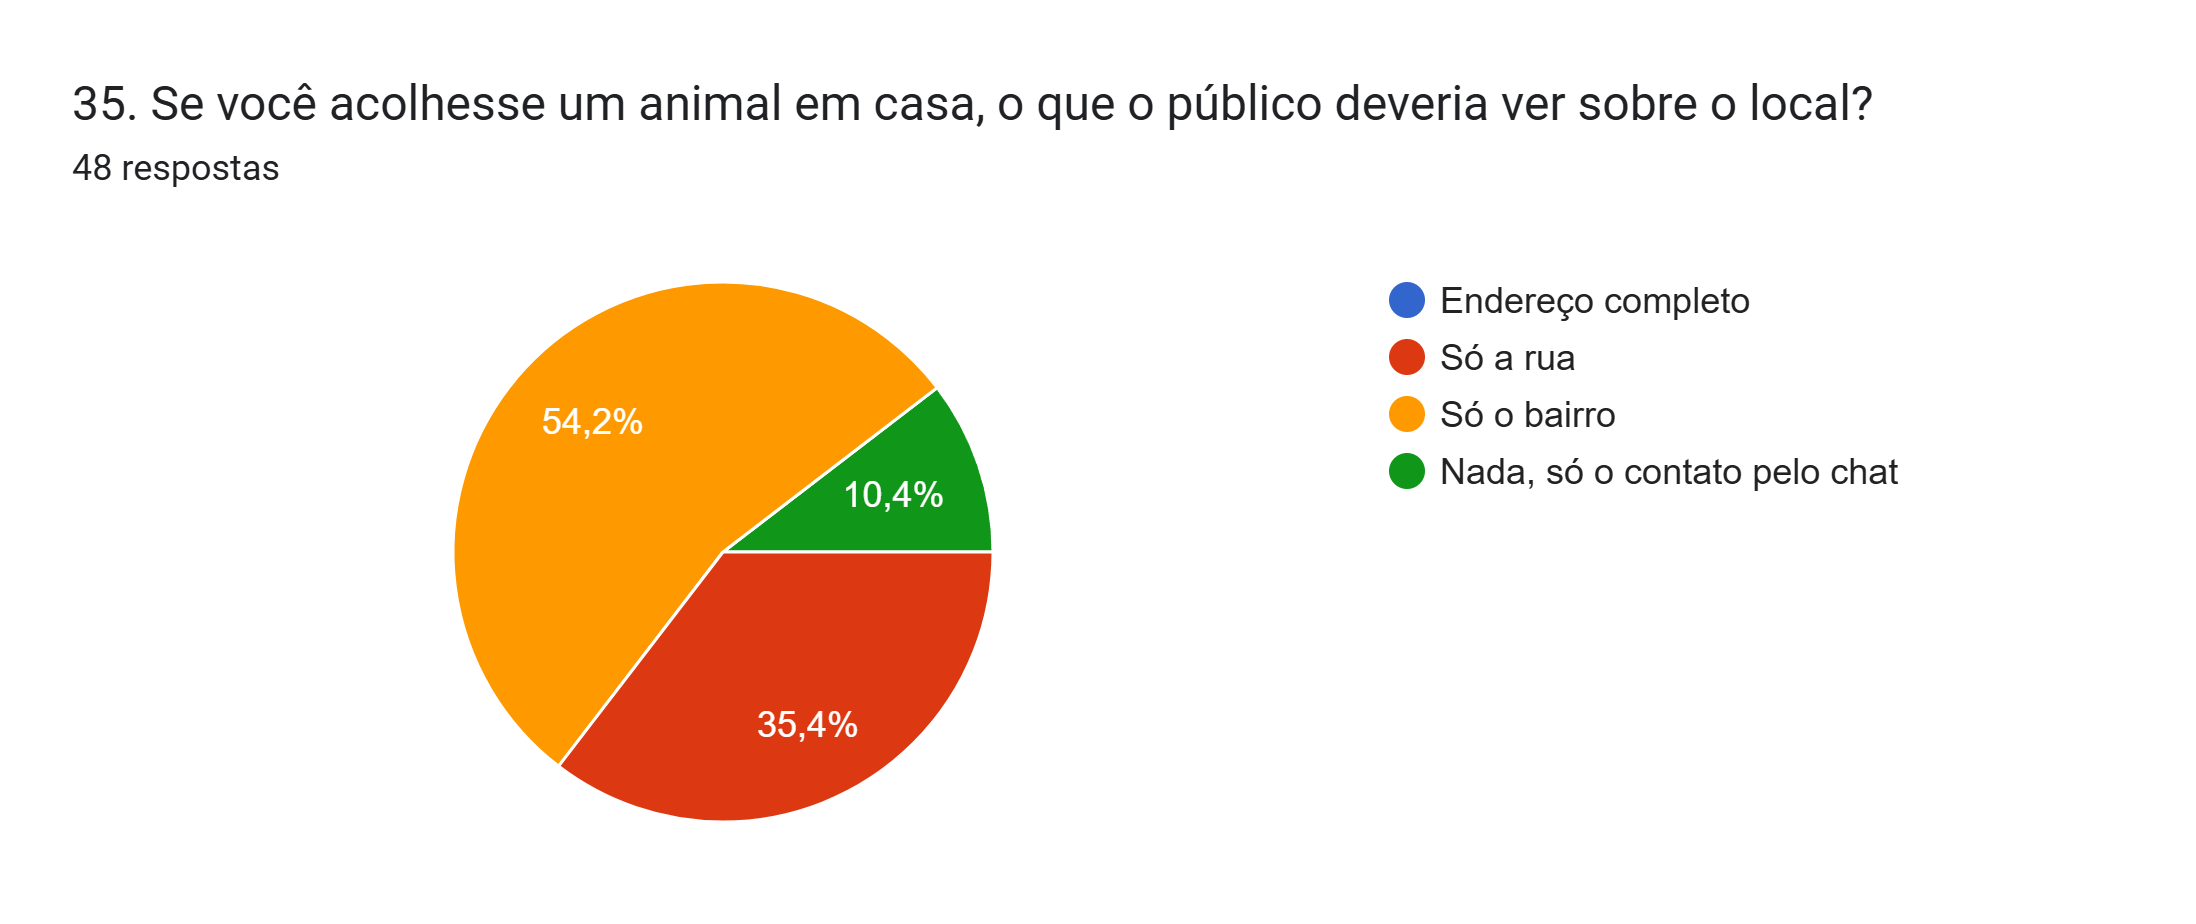
\includegraphics[width=\textwidth]{imagens/01_pesquisa/grafico_forms_q35_privacidade_local.png}
\fonte{Google Forms (2026).}
\end{figure}

Vinte e seis participantes (54,2\%) escolheriam exibir somente o bairro, 17 (35,4\%) somente a rua e cinco (10,4\%) não exibiriam o local, mantendo o contato pelo chat; ninguém escolheu mostrar o endereço completo.

No tema da convivência comunitária, 35 participantes (72,9\%) disseram já ter visto julgamentos em comentários de publicações sobre animais encontrados ou para doação; 36 (75\%) afirmaram que isso já lhes aconteceu pessoalmente. A publicação anônima foi aceita sem ressalvas por 21 (43,8\%), considerada conforme o caso por nove (18,8\%), rejeitada por 12 (25\%), que prefeririam aparecer, e rejeitada por seis (12,5\%). Sobre a devolução de um animal, todos pediriam prova de tutela: 32 sempre e 16 se desconfiassem da pessoa. Fotos antigas e detalhes conhecidos pelo tutor foram aceitos como evidência por 31 participantes cada; carteira de vacinação por 27, leitura do microchip por 26 e reação do animal por 26, com múltipla seleção. Vinte e seis (54,2\%) prefeririam um local público para a entrega ou busca do animal, 16 (33,3\%) uma clínica veterinária e seis (12,5\%) a própria casa. Para combinar o encontro no aplicativo, 28 (58,3\%) atribuíram notas 4 ou 5 e 20 (41,7\%), nota 3. A conversa prévia pelo chat foi selecionada como fator de confiança por 35 (72,9\%); fotos recentes por 32 (66,7\%), perfil com nome e foto por 31 (64,6\%) e avaliações de outras pessoas por 27 (56,3\%).

Na questão de avaliação das funcionalidades, os avisos automáticos de animais parecidos e a conversão do cadastro preventivo em alerta de animal perdido receberam notas 4 ou 5 de todos os 48 participantes. O cadastro preventivo com carteirinha digital obteve essas notas de 37 (77,1\%) e o cartaz com código QR, de 31 (64,6\%). A seção de adoção recebeu notas 4 ou 5 de 21 (43,8\%), enquanto 19 (39,6\%) deram nota 2; a oferta de recompensa recebeu nota 4 de 19 (39,6\%) e não teve nota 5. O lembrete de renovação após 30 dias recebeu nota 4 de 22 (45,8\%) e nota 3 de 26 (54,2\%). Portanto, as respostas indicam diferentes níveis de prioridade para os recursos. Na confirmação de uma possível correspondência, 23 participantes (47,9\%) prefeririam ver o animal pessoalmente, 17 (35,4\%) conversar com quem o encontrou e oito (16,7\%) comparar fotos e características; ninguém confiaria somente na sugestão do aplicativo.

As respostas finais também exigem interpretação sem extrapolação. Sobre o prazo para oferecer um animal à adoção após a busca pelo tutor, as respostas se distribuíram entre sete dias (17; 35,4\%), 15 dias (10; 20,8\%), 30 dias (10; 20,8\%) e nunca (11; 22,9\%); ninguém escolheu três dias. Esse item registra opiniões e não determina prazo legal ou procedimento de destinação. Quanto à recompensa, 16 participantes (33,3\%) responderam ``sim'', 14 (29,2\%) ``talvez'' e 18 (37,5\%) ``não''. Sobre instalar um aplicativo gratuito, 24 (50\%) o fariam assim que disponível, 19 (39,6\%) responderam ``talvez'' e cinco (10,4\%) somente se seu animal se perdesse; nenhum escolheu ``não''. O contato sem exposição do telefone foi a funcionalidade mais escolhida como diferencial (14; 29,2\%), seguido da rota (11; 22,9\%), dos avisos de avistamento (9; 18,8\%), do aviso de animal parecido (8; 16,7\%) e do mapa (6; 12,5\%). Por fim, 21 pessoas (43,8\%) aceitaram ser contatadas para testar o aplicativo em um formulário separado, e 27 (56,3\%) não aceitaram.

As perguntas abertas receberam 31 respostas na questão 15 e 40 na questão 51. Elas foram tratadas como material qualitativo complementar. Para preservar o anonimato, os relatos individuais não são reproduzidos. Os resultados quantitativos descrevem as pessoas que responderam ao formulário; não comprovam a eficácia do aplicativo nem substituem sua avaliação com usuários, apresentada no Capítulo 8.
